%!TEX root = ../main.tex

\chapter{Introduction\label{chap:introduction}}

\section{Motivation}

The digital content revolution has transformed journalism into a high-velocity industry where platforms must simultaneously manage exponential content growth and maintain rigorous quality standards. \cite{seznam2025} (~\reffig{fig:main_page}), serving over 5 million daily users, currently relies on human editors to manually assess only 20\% of submitted articles - an unsustainable practice given the platform's 50\% annual content growth rate. This manual process introduces significant challenges:
\begin{itemize}
  \item \textbf{Scalability limitations:} With article submissions increasing by 50\% annually, human editors cannot maintain pace without compromising review depth
  \item \textbf{Consistency issues:} Inter-editor agreement analysis reveals 20\% variance in quality ratings for identical content
  \item \textbf{Quality degradation risks:} Unreviewed articles risk platform credibility through potential misinformation or poorly structured content
\end{itemize}

These limitations highlight the need for more efficient and consistent methods for evaluating journalistic quality.
Automated quality classification addresses these challenges by providing:
\begin{itemize}
  \item Real-time assessment for 100\% of submissions
  \item Consistent application of editorial guidelines
  \item Significantly reduce the workload on human editors
  \item 24/7 operational capacity without human fatigue
  \item Data-driven insights for continuous quality improvement
\end{itemize}

Therefore, the primary motivation for this research is to develop an automated system capable of classifying the journalistic quality of articles, mimicking the complex decision-making process of experienced human editors.

\begin{figure}[htbp]
  \centering
  
\includegraphics[width=0.45\textwidth]{./fig/photos/Seznam_main_page.png}
  \caption{Example of Seznam.cz Homepage Displaying News Content}
  \label{fig:main_page}
\end{figure}

\begin{figure}
  \centering
  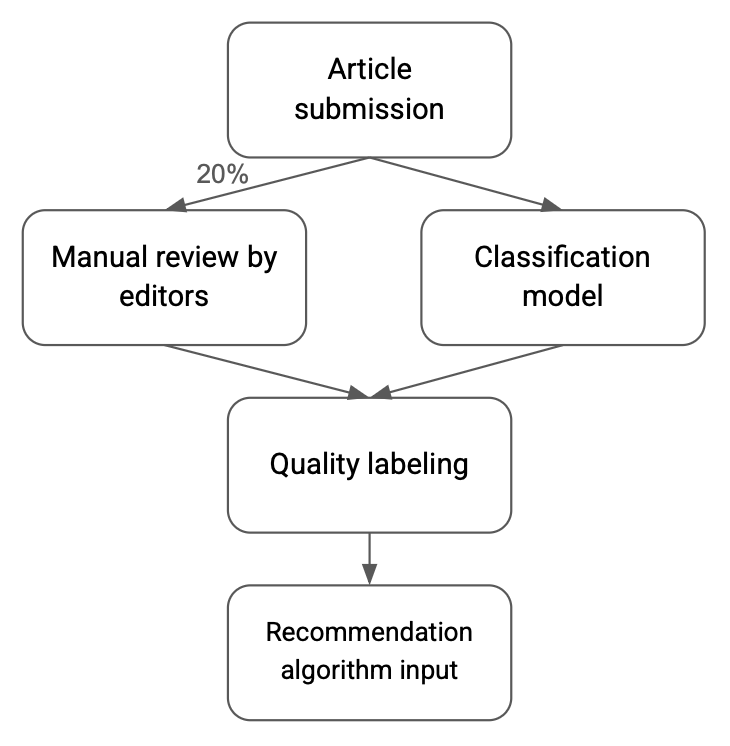
\includegraphics[width=0.5\textwidth]{./fig/photos/Current_Editorial_Workflow.png}
  \caption{Current Editorial Workflow}
  \label{fig:editor_workflow}
\end{figure}


\section{Problem Formulation}\label{sec:problem_formulation}
The core problem addressed in this thesis is the multi-class supervised classification of journalistic articles based on their quality. Our goal is to develop a computational model that automatically assigns an article to one of four predefined quality categories, reflecting the standards used by editors at Seznam.cz.

\begin{itemize}
  \item \ac{Class 0}: Low-quality content that lacks structure and depth.
  \item \ac{Class 1}: Lacks depth and analysis, often recycling
  known information with limited sources.
  \item \ac{Class 2}: Reliable news articles with at least five paragraphs and
  two references.
  \item \ac{Class 3}: Long, detailed, well-structured articles with visuals,
  subheadings, and references.
\end{itemize}

In the context of this thesis, \textbf{"journalistic quality"} is defined by a combination of factors that human editors consider. These include textual properties like readability, complexity, and style; structural attributes such as organization, paragraphing, and the use of headings; content characteristics like depth of analysis, factual accuracy, and source referencing; and metadata signals like the publishing channel. The aim is to create a model that learns to identify the patterns associated with these factors to predict the appropriate quality category. A significant challenge within this problem is the inherent imbalance in real-world data, where lower-quality categories are often much more frequent than the highest-quality ones.

\section{Structure of the Thesis}
This section provides an overview of the organization and content of the thesis. Chapter~\ref{chap:introduction} introduces the background, motivation, and problem formulation. It also reviews related work in journalistic quality assessment. 

Chapter~\ref{chap:data_collection} describes the data collection and analysis process. This chapter explains the sources of articles used in the study, the annotation process performed by human editors, and how the dataset is cleaned and prepared for analysis. It also reports basic statistics of the data and discusses strategies to address class imbalance. 

Chapter~\ref{chap:evaluation} covers the evaluation metrics used to assess the classification models. It explains why accuracy is not sufficient given the class imbalance. It describes metrics such as precision, recall, and F1 score to measure model performance. 

Chapter~\ref{chap:methodology} outlines the methodology of the thesis. It explains the overall approach to classifying article quality, including how baseline models are developed and how advanced models are used. It also discusses feature engineering, the use of pre-trained language models and \ac{CatBoost}, and how the models are trained and tuned. 

Chapter ~\ref{chap:experiments} presents the experiments and results. It describes the experimental setup and compares the performance of different classification models. It also shows the results of those models. 

Chapter ~\ref{chap:discussion} provides a discussion of the findings and suggests directions for future work. It interprets the results in the context of the research goals. It also considers possible improvements or extensions. 

Finally, Chapter ~\ref{chap:conclusion} concludes the thesis by summarizing the main contributions of the work. It outlines the overall conclusions of the study.

\clearpage
\section{Related Work}

The automated classification of journalistic quality is a multidisciplinary challenge that integrates \ac{NLP}, \ac{ML}, and media studies. This section critically reviews existing literature across these fields, highlighting significant contributions and identifying gaps that this thesis addresses, particularly in the context of the Czech language media environment and platforms like Seznam.cz.


\subsection{Quality Assessment Frameworks in Journalism}

Traditional journalistic quality assessment relies on human evaluation guided by professional standards. \cite{lacy2015} established eight core dimensions of journalistic quality, including accuracy, context, and sourcing diversity. While comprehensive, their framework was designed for manual evaluation, limiting its applicability to automated systems. Recent work by \cite{calvo2024} extends these principles to AI-assisted journalism, emphasizing transparency, accountability, and ethical considerations as critical criteria for maintaining quality in digital news production. Their study highlights that AI can enhance efficiency but risks reducing nuance and context, necessitating robust evaluation frameworks.

% https://www.jwac.org/Lacy.pdf
% Методы измерения качества журналистики
% Контент-анализ:
% Систематическое изучение публикаций по заданным критериям (например, сколько источников используется, насколько материал сбалансирован).
% Опросы аудитории:
% Изучение предпочтений и восприятия качества у читателей/зрителей.
% Экспертные оценки:
% Профессионалы или исследователи оценивают материалы по шкале качества.
% Косвенные показатели:
% Анализируется, например, уровень вовлечённости аудитории или влияние публикаций на общественную дискуссию.

\subsection{Computational Approaches to Text Quality Assessment}

Automated text quality assessment provides foundational insights for journalistic applications. \cite{pitler2008} demonstrated correlations between syntactic features and human perceptions of writing quality, using metrics like sentence complexity and coherence. However, their approach was general and did not address the specific stylistic and ethical requirements of journalistic texts. More recent advancements, as noted in a 2024 article by \cite{quantum2024}, leverage \ac{NLP} techniques such as grammar analysis, sentiment analysis, and text cohesion metrics to evaluate content quality automatically. These methods offer promising tools for journalism but require adaptation to domain-specific standards.

\subsection{Machine Learning for Classification of Media Content}

Machine learning has significantly advanced media content classification. \cite{potthast2018} developed methods to detect style-based bias in news articles, focusing on political orientation. Their work illustrates the potential of \ac{ML} to identify subtle textual patterns but does not directly address overall quality. Similarly, \cite{gonzalez2021} applied BERT-based architectures to classify news articles by credibility, achieving accuracy rates above 85\%. However, their binary classification approach (credible vs. non-credible) does not capture the nuanced spectrum of journalistic quality, which often requires multi-class models.

% https://ojs.aaai.org/index.php/AAAI/article/view/5386/5242
% Выводы
% Достоверность новостных статей действительно можно оценивать по стилю, но для этого нужны большие корпуса и продуманные процедуры обучения и тестирования, чтобы избежать переобучения на источники и темы.
% Стилометрические признаки и нейросетевые подходы — перспективное направление для автоматического выявления фейковых новостей.
% Интерпретируемость модели важна для доверия пользователей и дальнейшего развития методов.

% https://asu.elsevierpure.com/en/publications/stance-detection-with-bert-embeddings-for-credibility-analysis-of
% Впервые продемонстрировано, что комбинация BERT и stance-признаков позволяет достичь рекордной точности в детекции фейковых новостей.

\subsection{Multi-class Classification in Natural Language Processing}

Multi-class classification in \ac{NLP} is a critical technique for categorizing text into multiple predefined classes, making it highly relevant for assessing the quality of journalistic content across various dimensions, such as accuracy, depth, and balance. A comprehensive review by \cite{minaee2020} examines over 150 deep learning models applied to text classification tasks, including sentiment analysis, news categorization, and question answering. The authors highlight the effectiveness of transformer-based architectures, such as BERT and its variants, which leverage large-scale pretraining and fine-tuning to achieve state-of-the-art performance in complex multi-class classification problems. These models are particularly promising for evaluating journalistic quality, as they can capture semantic nuances and contextual relationships within news articles. The review also summarizes over 40 popular datasets, some of which focus on news categorization, providing valuable benchmarks for developing quality assessment systems.

Similarly, \cite{schmidt2019} introduced a multi-class approach for classifying Wikipedia article quality using document embeddings and content features. Their method, which achieved high accuracy in distinguishing quality levels, demonstrates the potential of semantic representations for quality assessment, adaptable to journalistic contexts.

% \subsection{AI in Journalism and Quality Implications}

% The integration of AI in journalism has transformed news production, as evidenced by recent studies. \cite{newman2025} report that 87\% of newsrooms have adopted generative AI for tasks like content creation (77\% deem it important) and automation. However, they note concerns about "AI slop" (low-quality AI-generated content) and the need for transparency, such as adopting C2PA metadata standards. A 2025 mini-review by \cite{frontiers2025} found that AI has revolutionized news production but poses ethical challenges, including reduced nuance in storytelling. These findings underscore the need for automated quality assessment tools that align with journalistic values.

\subsection{Linguistic Features for Quality Assessment}

Identifying linguistic features that correlate with quality is a key research area. \cite{schmidt2019} utilized document embeddings to capture semantic content, combined with features like section length and readability scores, to assess article quality. In journalism, similar features—such as Flesch-Kincaid readability, lexical diversity, and syntactic complexity—can indicate quality but must be tailored to journalistic standards. The Czech language, with its rich morphology and inflectional system, presents unique challenges for \ac{NLP} tools, as standard models designed for English may underperform.

\subsection{Research Gaps}
Despite progress, several gaps persist in the literature. First, most studies focus on English-language content, with limited exploration of languages like Czech, where morphological complexity affects \ac{NLP} performance. Second, many approaches rely on binary classification, which oversimplifies the multi-dimensional nature of journalistic quality. Third, few studies address the specific needs of news aggregation platforms like Seznam.cz, where high content volume and diversity demand scalable, language-specific solutions. Finally, ethical concerns, such as bias in AI models and the loss of human judgment, remain underexplored in automated quality assessment.

This thesis aims to address these gaps by developing a multi-class classification model tailored for the Czech language media environment. By integrating textual analysis, metadata, and Czech-specific linguistic features, this work builds on existing research while tackling its limitations, particularly for news aggregation platforms.

\section{Contributions}

\begin{itemize}
  \item A dataset of Czech articles annotated with four quality levels was prepared for multi-class classification. Texts were cleaned and filtered to ensure high-quality input data.
  \item Class imbalance in the dataset was mitigated by applying balancing techniques. Resampling of minority classes and class-weighting were used to improve model learning on underrepresented categories.
  \item Transformer-based language models, especially \ac{DeBERTaV3}, were fine-tuned to capture semantic and contextual cues relevant to article quality.
  \item A \ac{CatBoost} model was trained using a variety of linguistic and structural features, offering a non-transformer baseline for comparison.
  \item A hybrid classification model was developed by combining outputs from the transformer and \ac{CatBoost} models, improving predictive performance through model fusion.
  \item Evaluation was based on the weighted F1 score to fairly account for class imbalance, with the hybrid model achieving the best performance among all tested approaches.
  \item The thesis demonstrates that automated classification of article quality is feasible and can effectively support content assessment systems in high-volume environments.
\end{itemize}